% ============================================================
%  SAMLET RAPPORT -- Elektrisk Energisystem (62768)
%  Fælles præambel: preamble.tex
%  Hver sektionsfil kan også kompileres alene (se \ifdefined\mainfile).
%  Kompiler:  latexmk -pdf main.tex     (eller pdflatex main, 2x)
%  NB: \documentclass står her, så Overleaf vælger main.tex som hoveddokument.
% ============================================================
\documentclass{article}
% ============================================================
%  FÆLLES PRÆAMBEL
%  Deles af main.tex (hele rapporten) og de enkelte sektionsfiler,
%  som via \ifdefined\mainfile også kan kompileres alene.
%  Ret kun pakker/stil her ét sted.
%  NB: \documentclass er IKKE her -- den står i main.tex (og i sektionernes
%  standalone-guard), så Overleaf ikke forveksler preamble.tex med hoveddokumentet.
% ============================================================
\usepackage[utf8]{inputenc}
\usepackage[T1]{fontenc}
\usepackage[danish]{babel}
\usepackage{subcaption}
\usepackage{graphicx}              % Indsættelse af billeder
\usepackage[absolute,overlay]{textpos}
\usepackage{float}                 % H-placering
\usepackage{amsmath}
\usepackage{amssymb}
\usepackage{siunitx}               % \SI{15}{\volt} m.m. -- praktisk til måleresultater
\usepackage{booktabs}
\usepackage[a4paper, left=2.5cm, right=2.5cm, top=2.5cm, bottom=2.5cm]{geometry}
\usepackage{listings}              % Kildekode-listings
\usepackage{xcolor}
\usepackage{tikz}
\usetikzlibrary{automata, positioning, arrows, calc, shapes.geometric}
\tikzset{
    >=stealth,
    shorten >=2pt, shorten <=2pt,
    node distance=2.8cm,
    block/.style={draw, very thick, rectangle, minimum height=1cm, minimum width=2cm, fill=blue!10},
}
\usepackage[colorlinks=true,
            linkcolor=black,
            citecolor=blue,
            urlcolor=blue]{hyperref}

% ------------------------------------------------------------
%  Listing-stil til C / Arduino-firmware
% ------------------------------------------------------------
\lstdefinestyle{c}{
    language=C,
    basicstyle=\footnotesize\ttfamily,
    keywordstyle=\color{blue}\bfseries,
    commentstyle=\color{green!60!black}\itshape,
    stringstyle=\color{red},
    numbers=left, numberstyle=\tiny\color{gray}, stepnumber=1, numbersep=8pt,
    showspaces=false, showstringspaces=false, showtabs=false,
    frame=single, rulecolor=\color{black}, tabsize=4, captionpos=b,
    breaklines=true, breakatwhitespace=false,
    literate=%
        {æ}{{\ae}}1 {ø}{{\o}}1 {å}{{\aa}}1
        {Æ}{{\AE}}1 {Ø}{{\O}}1 {Å}{{\AA}}1,
}

% ------------------------------------------------------------
%  Listing-stil til MATLAB
% ------------------------------------------------------------
\lstdefinestyle{matlab}{
    language=Matlab,
    basicstyle=\footnotesize\ttfamily,
    keywordstyle=\color{blue}\bfseries,
    commentstyle=\color{green!60!black}\itshape,
    stringstyle=\color{magenta},
    numbers=left, numberstyle=\tiny\color{gray}, numbersep=8pt,
    showstringspaces=false, frame=single, tabsize=4, captionpos=b, breaklines=true,
}

\title{Elektrisk Energisystem}
\author{Gruppe \textbf{XX} -- 62768}
\date{Juni 2026}

% \mainfile defineres i main.tex (IKKE her) -- ellers tror standalone-sektioner
% også at de er i hoveddokumentet og springer deres \end{document} over.
\newcommand{\doubleunderline}[1]{\underline{\underline{#1}}}

\newcommand{\mainfile}{}   % markerer at sektionerne inkluderes -> spring standalone-guard over

\begin{document}

% ============================================================
%  FORSIDE (kun til den samlede rapport, main.tex)
% ============================================================

% Logo i højre hjørne
\begin{textblock*}{3cm}(17.5cm,1cm)
  
\includegraphics[scale=0.5]{images/frontpage/dtu_logo.png}
\end{textblock*}

\vspace*{3cm}
\begin{center}
    {\Huge \textbf{Elektrisk Energisystem}}\\[0.6cm]
    {\large Projektrapport}\\[1.5cm]
    \textbf{Kursus 62768 -- Electrical Energy Systems (projekt)}\\[0.3cm]
    Danmarks Tekniske Universitet \\
    Juni 2026
\end{center}

\vspace{2.5cm}

\begin{center}
\renewcommand{\arraystretch}{1.4}
\begin{tabular}{l l}
    \textbf{Navn} & \textbf{Studienr.} \\
    \hline
    Mads Rudolph        & s246132 \\
    \emph{Navn 2}       & \emph{sXXXXXX} \\
    \emph{Navn 3}       & \emph{sXXXXXX} \\
    \emph{Navn 4}       & \emph{sXXXXXX} \\
    \emph{Navn 5}       & \emph{sXXXXXX} \\
    \emph{Navn 6}       & \emph{sXXXXXX} \\
\end{tabular}
\end{center}

\vfill
\begin{center}
     \textbf{\large Gruppe XX}
\end{center}


% ============================================================
%  INDHOLD
% ============================================================
\newpage
\tableofcontents
\newpage

% ============================================================
%  RAPPORT
% ============================================================
\ifdefined\mainfile\else\documentclass{article}% ============================================================
%  FÆLLES PRÆAMBEL
%  Deles af main.tex (hele rapporten) og de enkelte sektionsfiler,
%  som via \ifdefined\mainfile også kan kompileres alene.
%  Ret kun pakker/stil her ét sted.
%  NB: \documentclass er IKKE her -- den står i main.tex (og i sektionernes
%  standalone-guard), så Overleaf ikke forveksler preamble.tex med hoveddokumentet.
% ============================================================
\usepackage[utf8]{inputenc}
\usepackage[T1]{fontenc}
\usepackage[danish]{babel}
\usepackage{subcaption}
\usepackage{graphicx}              % Indsættelse af billeder
\usepackage[absolute,overlay]{textpos}
\usepackage{float}                 % H-placering
\usepackage{amsmath}
\usepackage{amssymb}
\usepackage{siunitx}               % \SI{15}{\volt} m.m. -- praktisk til måleresultater
\usepackage{booktabs}
\usepackage[a4paper, left=2.5cm, right=2.5cm, top=2.5cm, bottom=2.5cm]{geometry}
\usepackage{listings}              % Kildekode-listings
\usepackage{xcolor}
\usepackage{tikz}
\usetikzlibrary{automata, positioning, arrows, calc, shapes.geometric}
\tikzset{
    >=stealth,
    shorten >=2pt, shorten <=2pt,
    node distance=2.8cm,
    block/.style={draw, very thick, rectangle, minimum height=1cm, minimum width=2cm, fill=blue!10},
}
\usepackage[colorlinks=true,
            linkcolor=black,
            citecolor=blue,
            urlcolor=blue]{hyperref}

% ------------------------------------------------------------
%  Listing-stil til C / Arduino-firmware
% ------------------------------------------------------------
\lstdefinestyle{c}{
    language=C,
    basicstyle=\footnotesize\ttfamily,
    keywordstyle=\color{blue}\bfseries,
    commentstyle=\color{green!60!black}\itshape,
    stringstyle=\color{red},
    numbers=left, numberstyle=\tiny\color{gray}, stepnumber=1, numbersep=8pt,
    showspaces=false, showstringspaces=false, showtabs=false,
    frame=single, rulecolor=\color{black}, tabsize=4, captionpos=b,
    breaklines=true, breakatwhitespace=false,
    literate=%
        {æ}{{\ae}}1 {ø}{{\o}}1 {å}{{\aa}}1
        {Æ}{{\AE}}1 {Ø}{{\O}}1 {Å}{{\AA}}1,
}

% ------------------------------------------------------------
%  Listing-stil til MATLAB
% ------------------------------------------------------------
\lstdefinestyle{matlab}{
    language=Matlab,
    basicstyle=\footnotesize\ttfamily,
    keywordstyle=\color{blue}\bfseries,
    commentstyle=\color{green!60!black}\itshape,
    stringstyle=\color{magenta},
    numbers=left, numberstyle=\tiny\color{gray}, numbersep=8pt,
    showstringspaces=false, frame=single, tabsize=4, captionpos=b, breaklines=true,
}

\title{Elektrisk Energisystem}
\author{Gruppe \textbf{XX} -- 62768}
\date{Juni 2026}

% \mainfile defineres i main.tex (IKKE her) -- ellers tror standalone-sektioner
% også at de er i hoveddokumentet og springer deres \end{document} over.
\newcommand{\doubleunderline}[1]{\underline{\underline{#1}}}
\begin{document}\fi

\section{Introduction}
\label{sec:intro}
% Kort: formålet med projektet (62768), hvad systemet skal kunne, og rapportens opbygning.
% Henvis til kravspecifikationen og det overordnede blokdiagram i afsnit~\ref{sec:systemoverblik}.

\noindent
Modern electrical energy systems often consist of several connected parts, such as energy sources, converters, storage units, control systems, and loads. The purpose of these systems is to deliver electrical energy in a stable and controlled way, even when the input source or the load changes. This is especially important when renewable energy sources, such as solar panels, are used, because their output depends on external conditions such as light intensity and temperature.

\vspace{0.4cm}

\noindent
In this project, a small-scale electrical energy system is designed and tested. The system includes an AC generator, a three-phase transformer, a rectifier, a PV module, MPPT control, buck and boost converters, and a load. The goal is to investigate how these components work together to produce, convert, regulate, and deliver electrical energy.

\vspace{0.4cm}

\noindent
A central part of the project is the use of power electronics. The rectifier converts AC voltage into DC voltage, while the buck and boost converters are used to regulate the voltage to the required levels. This is necessary because the voltage produced by the generator and the solar panel is not always directly suitable for the load.

\vspace{0.4cm}

\noindent
The system must fulfil several requirements. The rectified voltage from the AC-generator system must be regulated to approximately (15~\text{V}), and the system must be able to supply current to the buck converter. The final output voltage must also stay within the required limits during load changes. In addition, the system uses control and measurement circuits, where an Arduino can be used for voltage measurement, current measurement, PWM control, and MPPT implementation.

\vspace{0.4cm}

\noindent
The work in this project includes both theoretical analysis and practical measurements. First, the individual components are studied and tested separately. This includes measurements of the generator and rectifier output, measurements of the PV module I-V and P-V curves, and analysis of the maximum power point. Afterwards, the different parts of the system are combined and tested as a complete small-scale electrical energy system.

\vspace{0.4cm}

\noindent
The purpose of the report is to document the design, calculations, measurements, and testing of the electrical energy system. The report first presents the system overview and the main requirements. Afterwards, the different subsystems are explained, including the generator, transformer, rectifier, PV module, MPPT control, and power converters. Finally, the measured results are discussed and compared with the expected behaviour of the system.
 % TODO: skriv færdig.

\ifdefined\mainfile\else\end{document}\fi

\ifdefined\mainfile\else\documentclass{article}% ============================================================
%  FÆLLES PRÆAMBEL
%  Deles af main.tex (hele rapporten) og de enkelte sektionsfiler,
%  som via \ifdefined\mainfile også kan kompileres alene.
%  Ret kun pakker/stil her ét sted.
%  NB: \documentclass er IKKE her -- den står i main.tex (og i sektionernes
%  standalone-guard), så Overleaf ikke forveksler preamble.tex med hoveddokumentet.
% ============================================================
\usepackage[utf8]{inputenc}
\usepackage[T1]{fontenc}
\usepackage[danish]{babel}
\usepackage{subcaption}
\usepackage{graphicx}              % Indsættelse af billeder
\usepackage[absolute,overlay]{textpos}
\usepackage{float}                 % H-placering
\usepackage{amsmath}
\usepackage{amssymb}
\usepackage{siunitx}               % \SI{15}{\volt} m.m. -- praktisk til måleresultater
\usepackage{booktabs}
\usepackage[a4paper, left=2.5cm, right=2.5cm, top=2.5cm, bottom=2.5cm]{geometry}
\usepackage{listings}              % Kildekode-listings
\usepackage{xcolor}
\usepackage{tikz}
\usetikzlibrary{automata, positioning, arrows, calc, shapes.geometric}
\tikzset{
    >=stealth,
    shorten >=2pt, shorten <=2pt,
    node distance=2.8cm,
    block/.style={draw, very thick, rectangle, minimum height=1cm, minimum width=2cm, fill=blue!10},
}
\usepackage[colorlinks=true,
            linkcolor=black,
            citecolor=blue,
            urlcolor=blue]{hyperref}

% ------------------------------------------------------------
%  Listing-stil til C / Arduino-firmware
% ------------------------------------------------------------
\lstdefinestyle{c}{
    language=C,
    basicstyle=\footnotesize\ttfamily,
    keywordstyle=\color{blue}\bfseries,
    commentstyle=\color{green!60!black}\itshape,
    stringstyle=\color{red},
    numbers=left, numberstyle=\tiny\color{gray}, stepnumber=1, numbersep=8pt,
    showspaces=false, showstringspaces=false, showtabs=false,
    frame=single, rulecolor=\color{black}, tabsize=4, captionpos=b,
    breaklines=true, breakatwhitespace=false,
    literate=%
        {æ}{{\ae}}1 {ø}{{\o}}1 {å}{{\aa}}1
        {Æ}{{\AE}}1 {Ø}{{\O}}1 {Å}{{\AA}}1,
}

% ------------------------------------------------------------
%  Listing-stil til MATLAB
% ------------------------------------------------------------
\lstdefinestyle{matlab}{
    language=Matlab,
    basicstyle=\footnotesize\ttfamily,
    keywordstyle=\color{blue}\bfseries,
    commentstyle=\color{green!60!black}\itshape,
    stringstyle=\color{magenta},
    numbers=left, numberstyle=\tiny\color{gray}, numbersep=8pt,
    showstringspaces=false, frame=single, tabsize=4, captionpos=b, breaklines=true,
}

\title{Elektrisk Energisystem}
\author{Gruppe \textbf{XX} -- 62768}
\date{Juni 2026}

% \mainfile defineres i main.tex (IKKE her) -- ellers tror standalone-sektioner
% også at de er i hoveddokumentet og springer deres \end{document} over.
\newcommand{\doubleunderline}[1]{\underline{\underline{#1}}}
\begin{document}\fi

\section{System overview and requirements}
\label{sec:systemoverblik}
% Overordnet blokdiagram (se TikZ-skabelon nedenfor) + de vigtigste krav (V1/V2/V3).
% Forklar energistrømmen: AC-generator -> transformer -> ensretter -> buck;
% solcelle -> MPPT -> lineær reg -> energilager; boost -> pulserende last.

% --- Skabelon til blokdiagram (udfyld/erstat) ---
\begin{figure}[H]
    \centering
    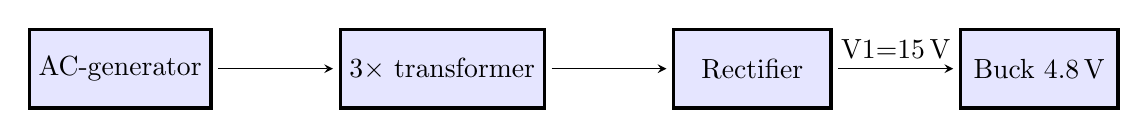
\begin{tikzpicture}[node distance=2.2cm and 1.6cm]
        \node[block] (gen)  {AC-generator};
        \node[block, right=of gen] (tr) {3$\times$ transformer};
        \node[block, right=of tr] (rec) {Rectifier};
        \node[block, right=of rec] (buck) {Buck 4.8\,V};
        \draw[->] (gen) -- (tr);
        \draw[->] (tr) -- (rec);
        \draw[->] (rec) -- node[above]{V1=15\,V} (buck);
    \end{tikzpicture}
    \caption{Simplified block diagram of the energy system, expanded with PV module/MPPT, energy storage, boost converter, and load).}
    \label{fig:blokdiagram}
\end{figure}

\begin{table}[H]
    \centering
    \begin{tabular}{c l l}
        \toprule
        \textbf{Node} & \textbf{Voltage} & \textbf{Requirement} \\
        \midrule
        V1 & 15\,V $\pm$1\,V  & at 100--300\,mA, hold within for 1.0\,s \\
        V2 & 10\,V $\pm$1\,V  & deliver $\geq$150\,mA, last-step 50--150\,mA \\
        V3 & 5\,V $\pm$0.5\,V & for currents $>$20\,mA \\
        \bottomrule
    \end{tabular}
    \caption{Central voltage specifications. Full list in appendiks~\ref{sec:kravsporing}.}
    \label{tab:krav-overblik}
\end{table}

\ifdefined\mainfile\else\end{document}\fi


\clearpage
\section{Delsystemer}
\ifdefined\mainfile\else\documentclass{article}% ============================================================
%  FÆLLES PRÆAMBEL
%  Deles af main.tex (hele rapporten) og de enkelte sektionsfiler,
%  som via \ifdefined\mainfile også kan kompileres alene.
%  Ret kun pakker/stil her ét sted.
%  NB: \documentclass er IKKE her -- den står i main.tex (og i sektionernes
%  standalone-guard), så Overleaf ikke forveksler preamble.tex med hoveddokumentet.
% ============================================================
\usepackage[utf8]{inputenc}
\usepackage[T1]{fontenc}
\usepackage[danish]{babel}
\usepackage{subcaption}
\usepackage{graphicx}              % Indsættelse af billeder
\usepackage[absolute,overlay]{textpos}
\usepackage{float}                 % H-placering
\usepackage{amsmath}
\usepackage{amssymb}
\usepackage{siunitx}               % \SI{15}{\volt} m.m. -- praktisk til måleresultater
\usepackage{booktabs}
\usepackage[a4paper, left=2.5cm, right=2.5cm, top=2.5cm, bottom=2.5cm]{geometry}
\usepackage{listings}              % Kildekode-listings
\usepackage{xcolor}
\usepackage{tikz}
\usetikzlibrary{automata, positioning, arrows, calc, shapes.geometric}
\tikzset{
    >=stealth,
    shorten >=2pt, shorten <=2pt,
    node distance=2.8cm,
    block/.style={draw, very thick, rectangle, minimum height=1cm, minimum width=2cm, fill=blue!10},
}
\usepackage[colorlinks=true,
            linkcolor=black,
            citecolor=blue,
            urlcolor=blue]{hyperref}

% ------------------------------------------------------------
%  Listing-stil til C / Arduino-firmware
% ------------------------------------------------------------
\lstdefinestyle{c}{
    language=C,
    basicstyle=\footnotesize\ttfamily,
    keywordstyle=\color{blue}\bfseries,
    commentstyle=\color{green!60!black}\itshape,
    stringstyle=\color{red},
    numbers=left, numberstyle=\tiny\color{gray}, stepnumber=1, numbersep=8pt,
    showspaces=false, showstringspaces=false, showtabs=false,
    frame=single, rulecolor=\color{black}, tabsize=4, captionpos=b,
    breaklines=true, breakatwhitespace=false,
    literate=%
        {æ}{{\ae}}1 {ø}{{\o}}1 {å}{{\aa}}1
        {Æ}{{\AE}}1 {Ø}{{\O}}1 {Å}{{\AA}}1,
}

% ------------------------------------------------------------
%  Listing-stil til MATLAB
% ------------------------------------------------------------
\lstdefinestyle{matlab}{
    language=Matlab,
    basicstyle=\footnotesize\ttfamily,
    keywordstyle=\color{blue}\bfseries,
    commentstyle=\color{green!60!black}\itshape,
    stringstyle=\color{magenta},
    numbers=left, numberstyle=\tiny\color{gray}, numbersep=8pt,
    showstringspaces=false, frame=single, tabsize=4, captionpos=b, breaklines=true,
}

\title{Elektrisk Energisystem}
\author{Gruppe \textbf{XX} -- 62768}
\date{Juni 2026}

% \mainfile defineres i main.tex (IKKE her) -- ellers tror standalone-sektioner
% også at de er i hoveddokumentet og springer deres \end{document} over.
\newcommand{\doubleunderline}[1]{\underline{\underline{#1}}}
\begin{document}\fi

\subsection{AC-generator, transformer og ensretter}
\label{sec:generator-transformer}
% Beskriv generatoren, 3-fase transformeren og ensretter + kondensator (15\,mF). Krav 1--3 (V1 = 15\,V). Inkl. simulering (Simulink) og målte resultater.

% TODO: design, beregninger, simulering, implementering og måleresultater.

\subsection*{DC-motor / AC-generator}

The system uses a Motraxx SR555SHP-3247S-75 brushed DC motor to drive an A20-22 L EVO kv924 three-phase generator. The DC motor has a rated voltage of \(12~\text{V}\) and a no-load speed of \(5887~\text{rpm}\). When the motor is loaded, the speed decreases to \(5024~\text{rpm}\), which shows that the connected generator and electrical load affect the motor speed. This is expected, since the motor must deliver mechanical torque to rotate the generator while the generator supplies electrical power to the rest of the system.

\noindent The speed drop of the DC motor can be calculated as:

\[
\Delta n = n_{\text{no-load}} - n_{\text{load}}
\]

\[
\Delta n = 5887 - 5024 = 863~\text{rpm}
\]

\noindent This corresponds to a percentage speed decrease of:

\[
\frac{863}{5887} \cdot 100 \approx 14.7\%
\]

\noindent This means that the motor speed decreases by approximately \(14.7\%\) when it is loaded.

\noindent The motor current also increases when the motor is loaded. The no-load current is \(0.25~\text{A}\), while the load current is \(1.46~\text{A}\). The current increase is therefore:

\[
\Delta I = I_{\text{load}} - I_{\text{no-load}}
\]

\[
\Delta I = 1.46 - 0.25 = 1.21~\text{A}
\]

\noindent The approximate electrical input power to the DC motor under load can be calculated as:

\[
P_{\text{in}} = V \cdot I
\]

\[
P_{\text{in}} = 12 \cdot 1.46 = 17.52~\text{W}
\]

\noindent So, under load, the DC motor uses approximately \(17.52~\text{W}\) of electrical input power.

\noindent The behavior of the DC motor can also be explained using the theory for a DC motor. The internal generated voltage, also called back EMF, is given by:

\[
E_A = K\phi\omega_m
\]

\noindent This equation shows that the internal generated voltage depends on the magnetic flux \(\phi\) and the mechanical speed \(\omega_m\). When the motor slows down, \(\omega_m\) decreases, and therefore the internal generated voltage \(E_A\) also decreases. The armature current is given by:

\[
I_A = \frac{V_T - E_A}{R_A}
\]

\noindent This means that when \(E_A\) decreases, the armature current \(I_A\) increases. The induced torque is given by:

\[
\tau_{\text{ind}} = K\phi I_A
\]

\noindent Therefore, when the armature current increases, the induced torque also increases. The motor then reaches a new operating point where the induced torque equals the load torque, but at a lower speed. This explains why the motor slows down when the generator is loaded and why it draws more current when more electrical power is required from the generator.
\vspace{0.5cm}

\noindent The generator is an A20-22 L EVO kv924 brushless outrunner motor. It is lightweight, weighing only \(55~\text{g}\), and has an operating voltage range of \(7.2~\text{V}\) to \(12.6~\text{V}\). According to the datasheet, the generator motor can run at around \(7200~\text{rpm}\) and has a power rating between \(165~\text{W}\) and \(187~\text{W}\), depending on the setup. This means that the generator motor is suitable for producing electrical energy in a small-scale energy system. In practice, the actual output voltage and current will depend on the speed of rotation, the load connected to the system, and losses in the transformer and rectifier.

\noindent Since the generator has a motor constant of \(924~\text{rpm/V}\), the approximate generated voltage at \(7200~\text{rpm}\) can be estimated as:

\[
V \approx \frac{n}{K_V}
\]

\[
V \approx \frac{7200}{924} \approx 7.79~\text{V}
\]

\noindent This is only an approximate value, because the actual generated voltage depends on the rotation speed, the connected load, the transformer connection, and losses in the rectifier.
\vspace{0.5cm}

\noindent In our system, the generated three-phase AC voltage is first connected through a \(Y-\Delta\) transformer and then through a three-phase rectifier. The transformer is used to adapt the three-phase voltage before it reaches the rectifier. The rectifier then converts the three-phase AC voltage into the DC voltage \(V_1\), which is used by the rest of the circuit.

\vspace{0.5cm}

\subsection*{Transformer}

Our transformer setup uses a Wye-to-Delta connection, written as \(Y-\Delta\). This means that the primary side of the transformer is connected in wye, while the secondary side is connected in delta. In our system, the transformer is placed between the three-phase generator and the three-phase rectifier. Its purpose is to adapt the generated AC voltage before it is converted into the DC voltage \(V_1\).
\vspace{0.5cm}
\noindent A three-phase transformer can either be made as one single three-phase transformer or as three separate single-phase transformers connected together. A single three-phase transformer is usually lighter, smaller, cheaper, and slightly more efficient. However, using three separate single-phase transformers can make maintenance easier, because one transformer can be replaced individually if there is a fault.

\noindent For a wye-connected primary side, the line voltage and phase voltage are related by:

\[
V_L = \sqrt{3} \cdot V_\phi
\]

\noindent This means that each transformer winding on the primary side only receives the phase voltage, which is smaller than the line-to-line voltage. On the delta-connected secondary side, the line voltage is equal to the phase voltage:

\[
V_L = V_\phi
\]

\noindent Because of this, the final voltage ratio depends both on the transformer turns ratio and on the \(Y-\Delta\) connection. If the transformer turns ratio is written as:

\[
a = \frac{V_{\phi,\text{primary}}}{V_{\phi,\text{secondary}}}
\]

\noindent then the line voltage relationship for a \(Y-\Delta\) transformer becomes:

\[
\frac{V_{L,\text{primary}}}{V_{L,\text{secondary}}}
=
\sqrt{3} \cdot a
\]

\noindent This means that the voltage on the secondary side is not only determined by the winding ratio, but also by the fact that the primary is connected in wye and the secondary is connected in delta.
\vspace{0.5cm}

\noindent Another important point is that three-phase transformer calculations are often done on a per-phase basis. This means that impedance, voltage regulation, efficiency, and similar calculations can be treated almost like single-phase transformer calculations, but applied to each phase of the three-phase system.
\vspace{0.5cm}

\noindent A useful advantage of the \(Y-\Delta\) transformer connection is that it helps reduce problems caused by third-harmonic components. In a pure wye-wye transformer, third-harmonic voltages can become large, especially if the load is unbalanced. In a \(Y-\Delta\) transformer, the delta winding gives these third-harmonic currents a closed path where they can circulate instead of appearing strongly in the output voltage. This helps make the voltage supplied to the rectifier more stable and reduces unwanted distortion.
\vspace{0.5cm}

\noindent The delta side can also help if the load is slightly unbalanced, because the delta connection can partly redistribute the imbalance between the phases. This makes the \(Y-\Delta\) connection more stable compared to some other transformer connections. Therefore, the \(Y-\Delta\) transformer is useful in our system because it affects the voltage level, improves stability, reduces harmonic problems, and helps provide a better three-phase AC input for the rectifier.


\subsection*{Rectifier}

\noindent
We use a three-phase diode rectifier consisting of six Schottky diodes. Three diodes are connected to the positive DC output, called the top diodes, and three diodes provide the return path to the negative output, called the bottom diodes. Each phase of the AC generator is connected to the rectifier input.

\vspace{0.4cm}

\noindent
At any instant, the phase with the highest voltage conducts through its corresponding top diode, while the phase with the lowest voltage provides the return path through one of the bottom diodes. In this way, the rectifier converts the three-phase AC input into a pulsating DC output. According to the lecture slides, two diodes conduct at the same time in a three-phase bridge rectifier, and each diode conducts for \(120^\circ\). The conducting diode pair is the pair connected between the two supply lines with the highest instantaneous line-to-line voltage.

\vspace{0.4cm}

\noindent
The line-to-line voltage is important for the rectifier, because the rectifier output depends on the voltage between two phases. For a three-phase system, the line-to-line voltage is related to the phase voltage by:

\[
V_L = \sqrt{3} \cdot V_\phi
\]

\vspace{0.2cm}

\noindent
Schottky diodes are chosen due to their low forward voltage drop, typically \(0.2~\text{V}\) to \(0.4~\text{V}\), which reduces power losses and increases the available DC voltage after rectification. This is useful because two diodes conduct at the same time, so the total diode voltage drop affects the final DC output voltage.

\vspace{0.5cm}

\noindent
After the rectifier, an RC filter is used to smooth the pulsating DC voltage. The capacitor stores charge during voltage peaks and releases it during voltage drops, reducing ripple and producing a more stable DC voltage. The lecture slides also mention that DC filters are usually made as \(L\), \(C\), or \(LC\) filters, and that the filter design depends on the harmonics and ripple content in the output voltage.

\vspace{0.5cm}

\noindent
The DC voltage after the rectifier is designed to operate in the range of approximately \(20\text{--}30~\text{V}\). This variation occurs due to changing load conditions in the system. When the load increases, more current is drawn, causing a voltage drop across internal resistances and components, which lowers the DC voltage. At lower load conditions, the voltage increases due to reduced current draw.

\vspace{0.5cm}

\noindent
This DC voltage is then fed into a buck converter, which steps the voltage down to a stable level of approximately \(15~\text{V}\) for the final load. The buck converter therefore converts a higher, variable input voltage into a lower and regulated output voltage.

\vspace{0.5cm}

\noindent
The load used during testing consists of a \(150~\Omega\) power resistor and a capacitor of \(15000~\mu\text{F}\). The resistor is implemented as a power resistor to safely dissipate the electrical power without overheating. At operating voltages between \(20~\text{V}\) and \(30~\text{V}\), the resistor draws a current between approximately \(133~\text{mA}\) and \(200~\text{mA}\).

\vspace{0.5cm}

\noindent
The maximum power dissipation at \(30~\text{V}\) is:

\[
P = \frac{V^2}{R}
\]

\[
P = \frac{30^2}{150} = 6~\text{W}
\]

\vspace{0.2cm}

\noindent
However, since the voltage is not constant and varies with load conditions, the average power dissipation is lower. A \(5~\text{W}\) power resistor can be acceptable for short or lower-voltage tests, but if the resistor is operated continuously near \(30~\text{V}\), a higher power rating such as \(10~\text{W}\) would be safer.

\vspace{0.5cm}

\noindent
The power resistor is used as a controllable test load to simulate the expected input conditions of the buck converter. Since the buck converter reduces the voltage from approximately \(20\text{--}30~\text{V}\) to \(15~\text{V}\), the input current is lower than the output current. The resistor is therefore selected to approximate the expected input current drawn by the buck converter during operation.

\vspace{0.5cm}

\noindent
Overall, the rectifier performance depends on values such as output voltage, output current, ripple content, diode current rating, peak current, and peak inverse voltage. These are important because the diodes must be able to handle the current and voltage stresses in the circuit.

\ifdefined\mainfile\else\end{document}\fi
   % AC-generator, 3x transformer, ensretter -> V1
\ifdefined\mainfile\else\documentclass{article}% ============================================================
%  FÆLLES PRÆAMBEL
%  Deles af main.tex (hele rapporten) og de enkelte sektionsfiler,
%  som via \ifdefined\mainfile også kan kompileres alene.
%  Ret kun pakker/stil her ét sted.
%  NB: \documentclass er IKKE her -- den står i main.tex (og i sektionernes
%  standalone-guard), så Overleaf ikke forveksler preamble.tex med hoveddokumentet.
% ============================================================
\usepackage[utf8]{inputenc}
\usepackage[T1]{fontenc}
\usepackage[danish]{babel}
\usepackage{subcaption}
\usepackage{graphicx}              % Indsættelse af billeder
\usepackage[absolute,overlay]{textpos}
\usepackage{float}                 % H-placering
\usepackage{amsmath}
\usepackage{amssymb}
\usepackage{siunitx}               % \SI{15}{\volt} m.m. -- praktisk til måleresultater
\usepackage{booktabs}
\usepackage[a4paper, left=2.5cm, right=2.5cm, top=2.5cm, bottom=2.5cm]{geometry}
\usepackage{listings}              % Kildekode-listings
\usepackage{xcolor}
\usepackage{tikz}
\usetikzlibrary{automata, positioning, arrows, calc, shapes.geometric}
\tikzset{
    >=stealth,
    shorten >=2pt, shorten <=2pt,
    node distance=2.8cm,
    block/.style={draw, very thick, rectangle, minimum height=1cm, minimum width=2cm, fill=blue!10},
}
\usepackage[colorlinks=true,
            linkcolor=black,
            citecolor=blue,
            urlcolor=blue]{hyperref}

% ------------------------------------------------------------
%  Listing-stil til C / Arduino-firmware
% ------------------------------------------------------------
\lstdefinestyle{c}{
    language=C,
    basicstyle=\footnotesize\ttfamily,
    keywordstyle=\color{blue}\bfseries,
    commentstyle=\color{green!60!black}\itshape,
    stringstyle=\color{red},
    numbers=left, numberstyle=\tiny\color{gray}, stepnumber=1, numbersep=8pt,
    showspaces=false, showstringspaces=false, showtabs=false,
    frame=single, rulecolor=\color{black}, tabsize=4, captionpos=b,
    breaklines=true, breakatwhitespace=false,
    literate=%
        {æ}{{\ae}}1 {ø}{{\o}}1 {å}{{\aa}}1
        {Æ}{{\AE}}1 {Ø}{{\O}}1 {Å}{{\AA}}1,
}

% ------------------------------------------------------------
%  Listing-stil til MATLAB
% ------------------------------------------------------------
\lstdefinestyle{matlab}{
    language=Matlab,
    basicstyle=\footnotesize\ttfamily,
    keywordstyle=\color{blue}\bfseries,
    commentstyle=\color{green!60!black}\itshape,
    stringstyle=\color{magenta},
    numbers=left, numberstyle=\tiny\color{gray}, numbersep=8pt,
    showstringspaces=false, frame=single, tabsize=4, captionpos=b, breaklines=true,
}

\title{Elektrisk Energisystem}
\author{Gruppe \textbf{XX} -- 62768}
\date{Juni 2026}

% \mainfile defineres i main.tex (IKKE her) -- ellers tror standalone-sektioner
% også at de er i hoveddokumentet og springer deres \end{document} over.
\newcommand{\doubleunderline}[1]{\underline{\underline{#1}}}
\begin{document}\fi

\subsection{Buck-converter}
\label{sec:buck}
The buck converter is designed to perform DC--DC conversion, with the primary purpose of stepping down the input voltage to a regulated 5 V DC level. This voltage is used by multiple components in the system, ensuring stable operation and providing protection to other electronics. For the same purpose, optocouplers are also implemented to keep the PWM source (primarily the MCU) separated from the other circuit. \\
\begin{figure}[H]
    \centering
    
\includegraphics[width=0.5\linewidth]{report/images/Buck/Buck_Reference.png}
    \caption{Buck Converter Reference}
    \label{fig:BuckRef}
\end{figure}
\noindent The circuit, shown in Figure~\ref{fig:BuckRef}, consists of a MOSFET (M), a diode (D), an inductor (L), and an output capacitor (C), forming a conventional buck converter layout. The MOSFET is driven by a PWM signal, which controls the duty cycle and thereby regulates the output voltage.\\
When the MOSFET is turned on, the input voltage $V_{in}$ is applied across the inductor, causing the inductor current to increase while storing energy in its magnetic field. During this phase, the diode is reverse-biased. When the MOSFET is turned off, the inductor current continues to flow through the diode, which becomes forward-biased, delivering energy to the load and maintaining current continuity. The capacitor smooths the output voltage by reducing ripple, while the resistor represents the load.\\
For the buck converter connected to the rectifier, an input voltage of approximately 15 V is expected. Under ideal conditions, the output voltage of a buck converter follows
\[
V_{out} = D \cdot V_{in},
\]
meaning that a duty cycle of approximately 33\% is required to obtain 5 V. Therefore, a fixed duty cycle of 33\% is implemented using a self designed PWM generator (see \ref{PWM_Buck}).\\
In contrast, the buck converter associated with the MPPT system requires a variable duty cycle. In this case, the PWM signal is generated and adjusted by the microcontroller (MCU), allowing dynamic control of the output voltage in order to optimize power extraction.

\begin{figure}[H]
    \centering
    
\includegraphics[width=1\linewidth]{report/images/Buck/Buck_with_PWM.png}
    \caption{Buck converter controlled by PWM circuit}
    \label{fig:PWM_Buck}
\end{figure}
% Selvbygget buck-konverter med diskrete komponenter (krav 8, 9, 12). Vout = 4.8\,V. Dimensionering af L og C, duty cycle, ripple, MOSFET-styring (IR2110, IRF540N).

% TODO: design, beregninger, simulering, implementering og måleresultater.

\ifdefined\mainfile\else\end{document}\fi
                     % Buck-konverter (Vout = 4.8 V)
\ifdefined\mainfile\else% ============================================================
%  FÆLLES PRÆAMBEL
%  Deles af main.tex (hele rapporten) og de enkelte sektionsfiler,
%  som via \ifdefined\mainfile også kan kompileres alene.
%  Ret kun pakker/stil her ét sted.
%  NB: \documentclass er IKKE her -- den står i main.tex (og i sektionernes
%  standalone-guard), så Overleaf ikke forveksler preamble.tex med hoveddokumentet.
% ============================================================
\usepackage[utf8]{inputenc}
\usepackage[T1]{fontenc}
\usepackage[danish]{babel}
\usepackage{subcaption}
\usepackage{graphicx}              % Indsættelse af billeder
\usepackage[absolute,overlay]{textpos}
\usepackage{float}                 % H-placering
\usepackage{amsmath}
\usepackage{amssymb}
\usepackage{siunitx}               % \SI{15}{\volt} m.m. -- praktisk til måleresultater
\usepackage{booktabs}
\usepackage[a4paper, left=2.5cm, right=2.5cm, top=2.5cm, bottom=2.5cm]{geometry}
\usepackage{listings}              % Kildekode-listings
\usepackage{xcolor}
\usepackage{tikz}
\usetikzlibrary{automata, positioning, arrows, calc, shapes.geometric}
\tikzset{
    >=stealth,
    shorten >=2pt, shorten <=2pt,
    node distance=2.8cm,
    block/.style={draw, very thick, rectangle, minimum height=1cm, minimum width=2cm, fill=blue!10},
}
\usepackage[colorlinks=true,
            linkcolor=black,
            citecolor=blue,
            urlcolor=blue]{hyperref}

% ------------------------------------------------------------
%  Listing-stil til C / Arduino-firmware
% ------------------------------------------------------------
\lstdefinestyle{c}{
    language=C,
    basicstyle=\footnotesize\ttfamily,
    keywordstyle=\color{blue}\bfseries,
    commentstyle=\color{green!60!black}\itshape,
    stringstyle=\color{red},
    numbers=left, numberstyle=\tiny\color{gray}, stepnumber=1, numbersep=8pt,
    showspaces=false, showstringspaces=false, showtabs=false,
    frame=single, rulecolor=\color{black}, tabsize=4, captionpos=b,
    breaklines=true, breakatwhitespace=false,
    literate=%
        {æ}{{\ae}}1 {ø}{{\o}}1 {å}{{\aa}}1
        {Æ}{{\AE}}1 {Ø}{{\O}}1 {Å}{{\AA}}1,
}

% ------------------------------------------------------------
%  Listing-stil til MATLAB
% ------------------------------------------------------------
\lstdefinestyle{matlab}{
    language=Matlab,
    basicstyle=\footnotesize\ttfamily,
    keywordstyle=\color{blue}\bfseries,
    commentstyle=\color{green!60!black}\itshape,
    stringstyle=\color{magenta},
    numbers=left, numberstyle=\tiny\color{gray}, numbersep=8pt,
    showstringspaces=false, frame=single, tabsize=4, captionpos=b, breaklines=true,
}

\title{Elektrisk Energisystem}
\author{Gruppe \textbf{XX} -- 62768}
\date{Juni 2026}

% \mainfile defineres i main.tex (IKKE her) -- ellers tror standalone-sektioner
% også at de er i hoveddokumentet og springer deres \end{document} over.
\newcommand{\doubleunderline}[1]{\underline{\underline{#1}}}
\begin{document}\fi

\subsection{Boost-konverter}
\label{sec:boost}
% Selvbygget boost-konverter til pulserende 10\,V last (krav 4--6, 8, 12). Dimensionering, regulering og last-respons.

% TODO: design, beregninger, simulering, implementering og måleresultater.

\ifdefined\mainfile\else\end{document}\fi
                    % Boost-konverter -> pulserende last (V2 = 10 V)
\ifdefined\mainfile\else\documentclass{article}% ============================================================
%  FÆLLES PRÆAMBEL
%  Deles af main.tex (hele rapporten) og de enkelte sektionsfiler,
%  som via \ifdefined\mainfile også kan kompileres alene.
%  Ret kun pakker/stil her ét sted.
%  NB: \documentclass er IKKE her -- den står i main.tex (og i sektionernes
%  standalone-guard), så Overleaf ikke forveksler preamble.tex med hoveddokumentet.
% ============================================================
\usepackage[utf8]{inputenc}
\usepackage[T1]{fontenc}
\usepackage[danish]{babel}
\usepackage{subcaption}
\usepackage{graphicx}              % Indsættelse af billeder
\usepackage[absolute,overlay]{textpos}
\usepackage{float}                 % H-placering
\usepackage{amsmath}
\usepackage{amssymb}
\usepackage{siunitx}               % \SI{15}{\volt} m.m. -- praktisk til måleresultater
\usepackage{booktabs}
\usepackage[a4paper, left=2.5cm, right=2.5cm, top=2.5cm, bottom=2.5cm]{geometry}
\usepackage{listings}              % Kildekode-listings
\usepackage{xcolor}
\usepackage{tikz}
\usetikzlibrary{automata, positioning, arrows, calc, shapes.geometric}
\tikzset{
    >=stealth,
    shorten >=2pt, shorten <=2pt,
    node distance=2.8cm,
    block/.style={draw, very thick, rectangle, minimum height=1cm, minimum width=2cm, fill=blue!10},
}
\usepackage[colorlinks=true,
            linkcolor=black,
            citecolor=blue,
            urlcolor=blue]{hyperref}

% ------------------------------------------------------------
%  Listing-stil til C / Arduino-firmware
% ------------------------------------------------------------
\lstdefinestyle{c}{
    language=C,
    basicstyle=\footnotesize\ttfamily,
    keywordstyle=\color{blue}\bfseries,
    commentstyle=\color{green!60!black}\itshape,
    stringstyle=\color{red},
    numbers=left, numberstyle=\tiny\color{gray}, stepnumber=1, numbersep=8pt,
    showspaces=false, showstringspaces=false, showtabs=false,
    frame=single, rulecolor=\color{black}, tabsize=4, captionpos=b,
    breaklines=true, breakatwhitespace=false,
    literate=%
        {æ}{{\ae}}1 {ø}{{\o}}1 {å}{{\aa}}1
        {Æ}{{\AE}}1 {Ø}{{\O}}1 {Å}{{\AA}}1,
}

% ------------------------------------------------------------
%  Listing-stil til MATLAB
% ------------------------------------------------------------
\lstdefinestyle{matlab}{
    language=Matlab,
    basicstyle=\footnotesize\ttfamily,
    keywordstyle=\color{blue}\bfseries,
    commentstyle=\color{green!60!black}\itshape,
    stringstyle=\color{magenta},
    numbers=left, numberstyle=\tiny\color{gray}, numbersep=8pt,
    showstringspaces=false, frame=single, tabsize=4, captionpos=b, breaklines=true,
}

\title{Elektrisk Energisystem}
\author{Gruppe \textbf{XX} -- 62768}
\date{Juni 2026}

% \mainfile defineres i main.tex (IKKE her) -- ellers tror standalone-sektioner
% også at de er i hoveddokumentet og springer deres \end{document} over.
\newcommand{\doubleunderline}[1]{\underline{\underline{#1}}}
\begin{document}\fi

\subsection{Solcelle, MPPT og energilager}
\label{sec:solcelle-mppt}
% Solcellepanel -> MPPT (15\,mF) -> lineær regulator (5\,V) -> energilager (1\,F). Krav 7, 9, 17 (V3 = 5\,V).

% TODO: design, beregninger, simulering, implementering og måleresultater.

\ifdefined\mainfile\else\end{document}\fi
            % Solcelle + MPPT + lineær regulator -> V3
\ifdefined\mainfile\else\documentclass{article}% ============================================================
%  FÆLLES PRÆAMBEL
%  Deles af main.tex (hele rapporten) og de enkelte sektionsfiler,
%  som via \ifdefined\mainfile også kan kompileres alene.
%  Ret kun pakker/stil her ét sted.
%  NB: \documentclass er IKKE her -- den står i main.tex (og i sektionernes
%  standalone-guard), så Overleaf ikke forveksler preamble.tex med hoveddokumentet.
% ============================================================
\usepackage[utf8]{inputenc}
\usepackage[T1]{fontenc}
\usepackage[danish]{babel}
\usepackage{subcaption}
\usepackage{graphicx}              % Indsættelse af billeder
\usepackage[absolute,overlay]{textpos}
\usepackage{float}                 % H-placering
\usepackage{amsmath}
\usepackage{amssymb}
\usepackage{siunitx}               % \SI{15}{\volt} m.m. -- praktisk til måleresultater
\usepackage{booktabs}
\usepackage[a4paper, left=2.5cm, right=2.5cm, top=2.5cm, bottom=2.5cm]{geometry}
\usepackage{listings}              % Kildekode-listings
\usepackage{xcolor}
\usepackage{tikz}
\usetikzlibrary{automata, positioning, arrows, calc, shapes.geometric}
\tikzset{
    >=stealth,
    shorten >=2pt, shorten <=2pt,
    node distance=2.8cm,
    block/.style={draw, very thick, rectangle, minimum height=1cm, minimum width=2cm, fill=blue!10},
}
\usepackage[colorlinks=true,
            linkcolor=black,
            citecolor=blue,
            urlcolor=blue]{hyperref}

% ------------------------------------------------------------
%  Listing-stil til C / Arduino-firmware
% ------------------------------------------------------------
\lstdefinestyle{c}{
    language=C,
    basicstyle=\footnotesize\ttfamily,
    keywordstyle=\color{blue}\bfseries,
    commentstyle=\color{green!60!black}\itshape,
    stringstyle=\color{red},
    numbers=left, numberstyle=\tiny\color{gray}, stepnumber=1, numbersep=8pt,
    showspaces=false, showstringspaces=false, showtabs=false,
    frame=single, rulecolor=\color{black}, tabsize=4, captionpos=b,
    breaklines=true, breakatwhitespace=false,
    literate=%
        {æ}{{\ae}}1 {ø}{{\o}}1 {å}{{\aa}}1
        {Æ}{{\AE}}1 {Ø}{{\O}}1 {Å}{{\AA}}1,
}

% ------------------------------------------------------------
%  Listing-stil til MATLAB
% ------------------------------------------------------------
\lstdefinestyle{matlab}{
    language=Matlab,
    basicstyle=\footnotesize\ttfamily,
    keywordstyle=\color{blue}\bfseries,
    commentstyle=\color{green!60!black}\itshape,
    stringstyle=\color{magenta},
    numbers=left, numberstyle=\tiny\color{gray}, numbersep=8pt,
    showstringspaces=false, frame=single, tabsize=4, captionpos=b, breaklines=true,
}

\title{Elektrisk Energisystem}
\author{Gruppe \textbf{XX} -- 62768}
\date{Juni 2026}

% \mainfile defineres i main.tex (IKKE her) -- ellers tror standalone-sektioner
% også at de er i hoveddokumentet og springer deres \end{document} over.
\newcommand{\doubleunderline}[1]{\underline{\underline{#1}}}
\begin{document}\fi

\subsection{Current measurements}
\label{sec:stroemmaaling}
% Strømmåling -- op-amps tilladt, ingen øvrige IC'er (krav 10). INA219 anvendt efter aftale.

\noindent
Current measurement is needed in two places in the system. First, the MPPT algorithm
needs the panel current in order to compute the PV power $P = V \cdot I$ and track the
maximum power point (see Section~\ref{sec:styring}). Second, the supply currents are
used to verify the operation of the complete system, in particular to show that the
solar panel offloads the motor--generator.

\vspace{0.5cm} \noindent
The underlying measurement principle is the same in all cases. A small \emph{shunt
resistor} is placed in series with the current path, and the voltage drop across it is
measured. By Ohm's law the current then follows directly as
\[
I = \frac{V_{\text{shunt}}}{R_{\text{shunt}}}.
\]
Because the shunt resistance is small, the inserted voltage drop is kept low, so the
measurement does not noticeably disturb the circuit. The shunt resistor itself is a
single passive component, and the differential voltage across it is what has to be
amplified and digitised.

\vspace{0.5cm} \noindent
On the PV side this measurement is implemented with an INA219 module, which contains a
$0.1~\Omega$ shunt resistor together with an instrumentation amplifier and a 12-bit
analog-to-digital converter. The module is configured for a $32~\text{V}$ bus range and
a $\pm 320~\text{mV}$ shunt range (gain $\div 8$), and its calibration register is set so
that the current and power registers read directly in amps and watts. The Arduino reads
the bus voltage, the shunt voltage and the resulting current from the INA219 over the
I\textsuperscript{2}C bus (pins A4/A5). The series shunt resistor, whose differential
voltage is amplified and converted, is the core of the measurement, and the same shunt
could equally be read by an op-amp difference amplifier ahead of the microcontroller
ADC.

\vspace{0.5cm} \noindent
In the MPPT control loop the INA219 returns the panel voltage and current in every
iteration, and these are multiplied to obtain the instantaneous PV power used by the
Perturb-and-Observe algorithm. The measured panel currents span the full operating
range of the module, from approximately $0.60~\text{A}$ near short circuit down to about
$0.05~\text{A}$ close to the open-circuit voltage, as listed in
Table~\ref{tab:pv_measurements}. The supply currents for the complete-system test were
read directly from the laboratory power supplies: the motor drew $1.412~\text{A}$ with
the solar panel inactive and $0.944~\text{A}$ with it active, a reduction of about
$33\%$, which confirms that the panel contributes power and reduces the load on the
motor--generator.

\ifdefined\mainfile\else\end{document}\fi
            % Strømmåling med diskrete komponenter
\ifdefined\mainfile\else\documentclass{article}% ============================================================
%  FÆLLES PRÆAMBEL
%  Deles af main.tex (hele rapporten) og de enkelte sektionsfiler,
%  som via \ifdefined\mainfile også kan kompileres alene.
%  Ret kun pakker/stil her ét sted.
%  NB: \documentclass er IKKE her -- den står i main.tex (og i sektionernes
%  standalone-guard), så Overleaf ikke forveksler preamble.tex med hoveddokumentet.
% ============================================================
\usepackage[utf8]{inputenc}
\usepackage[T1]{fontenc}
\usepackage[danish]{babel}
\usepackage{subcaption}
\usepackage{graphicx}              % Indsættelse af billeder
\usepackage[absolute,overlay]{textpos}
\usepackage{float}                 % H-placering
\usepackage{amsmath}
\usepackage{amssymb}
\usepackage{siunitx}               % \SI{15}{\volt} m.m. -- praktisk til måleresultater
\usepackage{booktabs}
\usepackage[a4paper, left=2.5cm, right=2.5cm, top=2.5cm, bottom=2.5cm]{geometry}
\usepackage{listings}              % Kildekode-listings
\usepackage{xcolor}
\usepackage{tikz}
\usetikzlibrary{automata, positioning, arrows, calc, shapes.geometric}
\tikzset{
    >=stealth,
    shorten >=2pt, shorten <=2pt,
    node distance=2.8cm,
    block/.style={draw, very thick, rectangle, minimum height=1cm, minimum width=2cm, fill=blue!10},
}
\usepackage[colorlinks=true,
            linkcolor=black,
            citecolor=blue,
            urlcolor=blue]{hyperref}

% ------------------------------------------------------------
%  Listing-stil til C / Arduino-firmware
% ------------------------------------------------------------
\lstdefinestyle{c}{
    language=C,
    basicstyle=\footnotesize\ttfamily,
    keywordstyle=\color{blue}\bfseries,
    commentstyle=\color{green!60!black}\itshape,
    stringstyle=\color{red},
    numbers=left, numberstyle=\tiny\color{gray}, stepnumber=1, numbersep=8pt,
    showspaces=false, showstringspaces=false, showtabs=false,
    frame=single, rulecolor=\color{black}, tabsize=4, captionpos=b,
    breaklines=true, breakatwhitespace=false,
    literate=%
        {æ}{{\ae}}1 {ø}{{\o}}1 {å}{{\aa}}1
        {Æ}{{\AE}}1 {Ø}{{\O}}1 {Å}{{\AA}}1,
}

% ------------------------------------------------------------
%  Listing-stil til MATLAB
% ------------------------------------------------------------
\lstdefinestyle{matlab}{
    language=Matlab,
    basicstyle=\footnotesize\ttfamily,
    keywordstyle=\color{blue}\bfseries,
    commentstyle=\color{green!60!black}\itshape,
    stringstyle=\color{magenta},
    numbers=left, numberstyle=\tiny\color{gray}, numbersep=8pt,
    showstringspaces=false, frame=single, tabsize=4, captionpos=b, breaklines=true,
}

\title{Elektrisk Energisystem}
\author{Gruppe \textbf{XX} -- 62768}
\date{Juni 2026}

% \mainfile defineres i main.tex (IKKE her) -- ellers tror standalone-sektioner
% også at de er i hoveddokumentet og springer deres \end{document} over.
\newcommand{\doubleunderline}[1]{\underline{\underline{#1}}}
\begin{document}\fi

\subsection{Styring og software (Arduino)}
\label{sec:styring}
% PID-regulering af motor via PWM-driver. Arduino ADC, timer-interrupts og PWM (krav 15, 18). PC-baseret overvågning, 1\,s opdatering (krav 13, 14).

% TODO: design, beregninger, simulering, implementering og måleresultater.

\ifdefined\mainfile\else\end{document}\fi
                  % Arduino: PID, ADC, timer, PWM, overvågning
\ifdefined\mainfile\else\documentclass{article}% ============================================================
%  FÆLLES PRÆAMBEL
%  Deles af main.tex (hele rapporten) og de enkelte sektionsfiler,
%  som via \ifdefined\mainfile også kan kompileres alene.
%  Ret kun pakker/stil her ét sted.
%  NB: \documentclass er IKKE her -- den står i main.tex (og i sektionernes
%  standalone-guard), så Overleaf ikke forveksler preamble.tex med hoveddokumentet.
% ============================================================
\usepackage[utf8]{inputenc}
\usepackage[T1]{fontenc}
\usepackage[danish]{babel}
\usepackage{subcaption}
\usepackage{graphicx}              % Indsættelse af billeder
\usepackage[absolute,overlay]{textpos}
\usepackage{float}                 % H-placering
\usepackage{amsmath}
\usepackage{amssymb}
\usepackage{siunitx}               % \SI{15}{\volt} m.m. -- praktisk til måleresultater
\usepackage{booktabs}
\usepackage[a4paper, left=2.5cm, right=2.5cm, top=2.5cm, bottom=2.5cm]{geometry}
\usepackage{listings}              % Kildekode-listings
\usepackage{xcolor}
\usepackage{tikz}
\usetikzlibrary{automata, positioning, arrows, calc, shapes.geometric}
\tikzset{
    >=stealth,
    shorten >=2pt, shorten <=2pt,
    node distance=2.8cm,
    block/.style={draw, very thick, rectangle, minimum height=1cm, minimum width=2cm, fill=blue!10},
}
\usepackage[colorlinks=true,
            linkcolor=black,
            citecolor=blue,
            urlcolor=blue]{hyperref}

% ------------------------------------------------------------
%  Listing-stil til C / Arduino-firmware
% ------------------------------------------------------------
\lstdefinestyle{c}{
    language=C,
    basicstyle=\footnotesize\ttfamily,
    keywordstyle=\color{blue}\bfseries,
    commentstyle=\color{green!60!black}\itshape,
    stringstyle=\color{red},
    numbers=left, numberstyle=\tiny\color{gray}, stepnumber=1, numbersep=8pt,
    showspaces=false, showstringspaces=false, showtabs=false,
    frame=single, rulecolor=\color{black}, tabsize=4, captionpos=b,
    breaklines=true, breakatwhitespace=false,
    literate=%
        {æ}{{\ae}}1 {ø}{{\o}}1 {å}{{\aa}}1
        {Æ}{{\AE}}1 {Ø}{{\O}}1 {Å}{{\AA}}1,
}

% ------------------------------------------------------------
%  Listing-stil til MATLAB
% ------------------------------------------------------------
\lstdefinestyle{matlab}{
    language=Matlab,
    basicstyle=\footnotesize\ttfamily,
    keywordstyle=\color{blue}\bfseries,
    commentstyle=\color{green!60!black}\itshape,
    stringstyle=\color{magenta},
    numbers=left, numberstyle=\tiny\color{gray}, numbersep=8pt,
    showstringspaces=false, frame=single, tabsize=4, captionpos=b, breaklines=true,
}

\title{Elektrisk Energisystem}
\author{Gruppe \textbf{XX} -- 62768}
\date{Juni 2026}

% \mainfile defineres i main.tex (IKKE her) -- ellers tror standalone-sektioner
% også at de er i hoveddokumentet og springer deres \end{document} over.
\newcommand{\doubleunderline}[1]{\underline{\underline{#1}}}
\begin{document}\fi

\subsection{Drive Circuit}
\label{sec:DriveCircuit}


\noindent
The driver circuit is used to control the DC motor that drives the three-phase generator in the energy system. The motor speed is controlled by applying a PWM signal to the driver circuit. By changing the PWM duty cycle, the average voltage applied to the motor changes, which makes it possible to regulate the generator speed and therefore the generated voltage.

\vspace{0.4cm}

\noindent
In this project, the driver circuit consists of a CNY17 optocoupler, an IR2110 gate driver, and an IRF540N MOSFET. The circuit is designed to allow a low-voltage microcontroller signal to control a higher-power motor circuit. The microcontroller generates the PWM signal, while the MOSFET switches the motor current on and off.

\vspace{0.5cm}

\begin{figure}[H]
\centering

\includegraphics[width=0.90\textwidth]{report/images/DriveCircuit/Drivecircuit-KiCad.png}
\caption{KiCad schematic of the motor driver circuit used in the project.}
\label{fig:driver_circuit_KiCad}
\end{figure}

\vspace{0.5cm}

\noindent
The PWM signal from the microcontroller is first sent through the CNY17 optocoupler. The purpose of the optocoupler is to provide galvanic isolation between the low-voltage control side and the motor power side. This is important because the motor and generator can create electrical noise, voltage spikes, and ground potential differences. The optocoupler helps protect the microcontroller from these disturbances.

\vspace{0.4cm}

\noindent
The input side of the CNY17 contains an internal LED. A series resistor is used to limit the current through this LED and prevent damage. When the microcontroller sends a PWM signal, the LED inside the optocoupler turns on and off. On the output side of the optocoupler, this signal is transferred optically and used as the input signal for the IR2110 gate driver.

\vspace{0.4cm}

\noindent
The IR2110 is used as a MOSFET gate driver. A microcontroller output pin cannot normally supply enough current to charge and discharge the MOSFET gate quickly. Therefore, the IR2110 is used to amplify the control signal and provide a stronger gate drive signal to the MOSFET. This allows the MOSFET to switch faster and more reliably.

\vspace{0.4cm}

\noindent
In this circuit, the IR2110 is mainly used to drive the low-side MOSFET. The MOSFET used is an IRF540N N-channel MOSFET. The motor is connected between the positive supply and the drain of the MOSFET, while the source of the MOSFET is connected to ground. When the PWM signal turns the MOSFET on, current flows through the motor and the MOSFET to ground. When the MOSFET turns off, the motor current is interrupted.

\vspace{0.4cm}

\noindent
A flyback diode is placed across the motor. This diode is important because the motor is an inductive load. When the MOSFET turns off, the motor inductance tries to keep the current flowing, which can create a large voltage spike. The flyback diode gives this current a safe path and helps protect the MOSFET from overvoltage.

\vspace{0.4cm}

\noindent
The circuit also includes resistors around the MOSFET gate. These resistors help control the switching behaviour of the MOSFET. A gate resistor limits the peak gate current and reduces ringing during switching. A gate-to-source resistor is also used to make sure the MOSFET stays off when no valid gate signal is present. This prevents unintended switching of the motor.

\vspace{0.4cm}

\noindent
Decoupling capacitors are placed close to the IR2110 supply pins. These capacitors help stabilize the driver supply voltage and reduce the effect of switching noise. This is important because the MOSFET gate driver needs a stable supply voltage to operate reliably.

\vspace{0.5cm}

\begin{figure}[H]
\centering

\includegraphics[width=0.70\textwidth]{report/images/DriveCircuit/DriveCircuit-Hulprint.jpg}
\caption{Physical implementation of the motor driver circuit on perfboard.}
\label{fig:driver_circuit_physical}
\end{figure}

\vspace{0.5cm}

\noindent
The driver circuit is used as part of the generator control system. By changing the PWM duty cycle, the controller can adjust the speed of the DC motor. A higher duty cycle gives a higher average motor voltage, which increases the motor speed and generator output voltage. A lower duty cycle reduces the motor voltage, which lowers the generator speed and output voltage.

\vspace{0.4cm}

\noindent
Overall, the driver circuit provides a safe and reliable interface between the microcontroller and the DC motor. The CNY17 optocoupler provides galvanic isolation, the IR2110 provides sufficient gate drive current, and the IRF540N MOSFET switches the motor current. This makes the circuit suitable for controlling the motor-generator part of the electrical energy system using PWM.


\ifdefined\mainfile\else\end{document}\fi

\ifdefined\mainfile\else\documentclass{article}% ============================================================
%  FÆLLES PRÆAMBEL
%  Deles af main.tex (hele rapporten) og de enkelte sektionsfiler,
%  som via \ifdefined\mainfile også kan kompileres alene.
%  Ret kun pakker/stil her ét sted.
%  NB: \documentclass er IKKE her -- den står i main.tex (og i sektionernes
%  standalone-guard), så Overleaf ikke forveksler preamble.tex med hoveddokumentet.
% ============================================================
\usepackage[utf8]{inputenc}
\usepackage[T1]{fontenc}
\usepackage[danish]{babel}
\usepackage{subcaption}
\usepackage{graphicx}              % Indsættelse af billeder
\usepackage[absolute,overlay]{textpos}
\usepackage{float}                 % H-placering
\usepackage{amsmath}
\usepackage{amssymb}
\usepackage{siunitx}               % \SI{15}{\volt} m.m. -- praktisk til måleresultater
\usepackage{booktabs}
\usepackage[a4paper, left=2.5cm, right=2.5cm, top=2.5cm, bottom=2.5cm]{geometry}
\usepackage{listings}              % Kildekode-listings
\usepackage{xcolor}
\usepackage{tikz}
\usetikzlibrary{automata, positioning, arrows, calc, shapes.geometric}
\tikzset{
    >=stealth,
    shorten >=2pt, shorten <=2pt,
    node distance=2.8cm,
    block/.style={draw, very thick, rectangle, minimum height=1cm, minimum width=2cm, fill=blue!10},
}
\usepackage[colorlinks=true,
            linkcolor=black,
            citecolor=blue,
            urlcolor=blue]{hyperref}

% ------------------------------------------------------------
%  Listing-stil til C / Arduino-firmware
% ------------------------------------------------------------
\lstdefinestyle{c}{
    language=C,
    basicstyle=\footnotesize\ttfamily,
    keywordstyle=\color{blue}\bfseries,
    commentstyle=\color{green!60!black}\itshape,
    stringstyle=\color{red},
    numbers=left, numberstyle=\tiny\color{gray}, stepnumber=1, numbersep=8pt,
    showspaces=false, showstringspaces=false, showtabs=false,
    frame=single, rulecolor=\color{black}, tabsize=4, captionpos=b,
    breaklines=true, breakatwhitespace=false,
    literate=%
        {æ}{{\ae}}1 {ø}{{\o}}1 {å}{{\aa}}1
        {Æ}{{\AE}}1 {Ø}{{\O}}1 {Å}{{\AA}}1,
}

% ------------------------------------------------------------
%  Listing-stil til MATLAB
% ------------------------------------------------------------
\lstdefinestyle{matlab}{
    language=Matlab,
    basicstyle=\footnotesize\ttfamily,
    keywordstyle=\color{blue}\bfseries,
    commentstyle=\color{green!60!black}\itshape,
    stringstyle=\color{magenta},
    numbers=left, numberstyle=\tiny\color{gray}, numbersep=8pt,
    showstringspaces=false, frame=single, tabsize=4, captionpos=b, breaklines=true,
}

\title{Elektrisk Energisystem}
\author{Gruppe \textbf{XX} -- 62768}
\date{Juni 2026}

% \mainfile defineres i main.tex (IKKE her) -- ellers tror standalone-sektioner
% også at de er i hoveddokumentet og springer deres \end{document} over.
\newcommand{\doubleunderline}[1]{\underline{\underline{#1}}}
\begin{document}\fi

\subsection{Feedback circuit}
\label{sec:Feedback-circuit}

\subsection*{Optically Isolated Feedback Circuit}

\noindent
In this project, a feedback circuit is used to measure voltages from the power side of the system and transfer the measurement safely to the low-voltage control side. The control system uses a microcontroller to measure voltages and currents and to adjust the PWM duty cycle for the converters. Since the power circuit can contain higher voltages and switching noise, it is important to protect the microcontroller input and avoid a direct electrical connection between the power side and the control side.

\vspace{0.5cm}

\begin{figure}[H]
\centering

\includegraphics[width=0.90\textwidth]{report/images/Feedback-circuit/Feedback circuit.png}
\caption{KiCad schematic of the optically isolated feedback circuit. - Lecture 2, Exp 3A}
\label{fig:feedback_circuit_schematic}
\end{figure}

\vspace{0.5cm}

\noindent
For this reason, an optically isolated linear feedback circuit is used. The circuit is based on the IL300 linear optocoupler. The purpose of the IL300 is to transfer an analog voltage signal across a galvanic isolation barrier. This means that the measurement signal can be transferred from the power electronics circuit to the controller circuit without the two sides sharing the same electrical connection.

\vspace{0.4cm}

\noindent
The IL300 contains one LED and two matched photodiodes. On the input side, an MCP601 operational amplifier drives the LED inside the optocoupler. One of the photodiodes is used as feedback to the input-side op-amp. This feedback makes the LED current more proportional to the measured input voltage and helps reduce the non-linear behaviour of the LED. This is important because the signal must remain as linear as possible for the controller to use it correctly.

\vspace{0.4cm}

\noindent
The second photodiode is placed on the isolated output side. This photodiode receives the optical signal from the LED and produces a small current. This current is then converted back into a voltage using another MCP601 operational amplifier. The resulting voltage is a scaled version of the measured input voltage and can be connected to the ADC input of the microcontroller.

\vspace{0.5cm}

\begin{figure}[H]
\centering

\includegraphics[width=0.65\textwidth]{report/images/Feedback-circuit/Feedback circuit hulprint.png}
\caption{Practical implementation of the feedback circuit on perfboard.}
\label{fig:feedback_circuit_hulprint}
\end{figure}

\vspace{0.5cm}

\noindent
The feedback circuit is designed so that the measured voltage is scaled down to a safe level for the controller. The microcontroller ADC can measure voltages in the range of approximately (0-3.3~\text{V}), so the voltage from the power circuit must be reduced before it is used by the controller. In this circuit, the scaling is mainly determined by the input voltage divider and the op-amp feedback network.

\vspace{0.4cm}

\noindent
A voltage divider is used to create a reference voltage for the non-inverting input of the first MCP601 operational amplifier. The reference voltage can be calculated as:

\[
V_{\text{ref}} = V_{\text{in}} \cdot \frac{R_2}{R_1 + R_2}
\]

\noindent
Using \(R_1 = 10~\text{k}\Omega\), \(R_2 = 2~\text{k}\Omega\), and \(V_{\text{in}} = 20~\text{V}\), the scaled voltage becomes:

\[
V_{\text{ref}} = 20 \cdot \frac{2}{10+2}
\]

\[
V_{\text{ref}} \approx 3.33~\text{V}
\]


\noindent
This means that when the measured voltage is around (20~\text{V}), the reference voltage becomes approximately (3.33~\text{V}). This value is suitable for a (3.3~\text{V}) ADC input. It is important to note that this value is not the original power circuit voltage, but a scaled measurement signal that represents the higher voltage in a safe range.

\vspace{0.4cm}

\noindent
The (3.33~\text{V}) reference voltage is not directly copied to the isolated output side. Instead, it is used as a reference for the first op-amp stage. The MCP601 regulates the current through the IL300 optocoupler LED so that the inverting and non-inverting inputs of the op-amp are kept at approximately the same voltage. In this way, the op-amp controls the LED current and makes the optical signal proportional to the measured voltage.

\vspace{0.4cm}

\noindent
The feedback network around the first op-amp sets the gain of this stage. Using the resistor values in the circuit, the gain is:

\[
\begin{aligned}
A_{U3} &= -\frac{R_3}{R_2} \\
A_{U3} &= -\frac{33~\text{k}\Omega}{2~\text{k}\Omega} \\
A_{U3} &= -16.5
\end{aligned}
\]

\noindent
The negative sign shows that the stage is inverting. In practice, the op-amp output does not simply become (3.3~\text{V}). Instead, it outputs the voltage required to drive the correct LED current through the series resistor and the IL300 LED. During testing, the op-amp drive voltage was measured to be approximately (3.8~\text{V}). This is expected, because this voltage is used to control the optocoupler LED current and is not the voltage sent directly to the ADC.

\vspace{0.4cm}

\noindent
On the isolated side, the second MCP601 is used as a transimpedance amplifier. This converts the photodiode current from the IL300 into a voltage signal. This voltage is the isolated measurement signal that is sent to the microcontroller ADC. The purpose of this stage is to reproduce a scaled version of the measured voltage while maintaining galvanic isolation between the power circuit and the control circuit.

\vspace{0.4cm}

\noindent
The feedback signal can be used by the controller to monitor the voltage in the system. For example, it can be used to measure the generator output voltage, the rectified DC voltage, or the converter output voltage. Based on this measurement, the controller can adjust the PWM duty cycle to regulate the voltage. In this way, the feedback circuit becomes an important part of the closed-loop control system.

\vspace{0.4cm}


\begin{figure}[H]
\centering

\includegraphics[width=0.65\textwidth]{report/images/Feedback-circuit/Feedback_Output.png}
\caption{Oscilloscope measurement of the feedback output. - Project 3 report, 62783}
\label{fig:feedback_circuit_hulprint}
\end{figure}


\noindent
The oscilloscope measurement verifies the operation of the feedback circuit. The isolated output signal is stable and close to the expected ADC voltage level. The measured output is approximately (3.3~\text{V}), while the op-amp drive side is approximately (3.8~\text{V}). This confirms that the circuit successfully scales the measured voltage down to a safe voltage level for the microcontroller ADC. The small visible variations are mainly caused by switching noise and measurement noise, but they remain small enough that they do not significantly affect the control signal.

\vspace{0.4cm}

\noindent
Overall, the optically isolated feedback circuit is used to make voltage measurements safer and more reliable. It protects the microcontroller from higher voltages, reduces the risk of ground loops, and separates the noisy power electronics from the low-voltage control circuit. The IL300 linear optocoupler transfers the measurement signal across the galvanic isolation barrier, while the op-amp stages ensure that the signal is scaled and converted to a voltage level suitable for the ADC. This makes the circuit suitable for use in the energy system, where measured voltage signals are needed for regulation, monitoring, and PWM control.

\vspace{0.4cm}

\noindent
It should be noted that this feedback circuit is inspired by an earlier project, \textit{62783 Project 3. sem, Winter 2026}, where a similar optically isolated feedback circuit was designed and tested. The circuit has therefore been reused and adapted for this project, since it provides a suitable method for transferring voltage measurements safely from the power electronics side to the low-voltage controller side.


\ifdefined\mainfile\else\end{document}\fi


\clearpage
\ifdefined\mainfile\else\documentclass{article}% ============================================================
%  FÆLLES PRÆAMBEL
%  Deles af main.tex (hele rapporten) og de enkelte sektionsfiler,
%  som via \ifdefined\mainfile også kan kompileres alene.
%  Ret kun pakker/stil her ét sted.
%  NB: \documentclass er IKKE her -- den står i main.tex (og i sektionernes
%  standalone-guard), så Overleaf ikke forveksler preamble.tex med hoveddokumentet.
% ============================================================
\usepackage[utf8]{inputenc}
\usepackage[T1]{fontenc}
\usepackage[danish]{babel}
\usepackage{subcaption}
\usepackage{graphicx}              % Indsættelse af billeder
\usepackage[absolute,overlay]{textpos}
\usepackage{float}                 % H-placering
\usepackage{amsmath}
\usepackage{amssymb}
\usepackage{siunitx}               % \SI{15}{\volt} m.m. -- praktisk til måleresultater
\usepackage{booktabs}
\usepackage[a4paper, left=2.5cm, right=2.5cm, top=2.5cm, bottom=2.5cm]{geometry}
\usepackage{listings}              % Kildekode-listings
\usepackage{xcolor}
\usepackage{tikz}
\usetikzlibrary{automata, positioning, arrows, calc, shapes.geometric}
\tikzset{
    >=stealth,
    shorten >=2pt, shorten <=2pt,
    node distance=2.8cm,
    block/.style={draw, very thick, rectangle, minimum height=1cm, minimum width=2cm, fill=blue!10},
}
\usepackage[colorlinks=true,
            linkcolor=black,
            citecolor=blue,
            urlcolor=blue]{hyperref}

% ------------------------------------------------------------
%  Listing-stil til C / Arduino-firmware
% ------------------------------------------------------------
\lstdefinestyle{c}{
    language=C,
    basicstyle=\footnotesize\ttfamily,
    keywordstyle=\color{blue}\bfseries,
    commentstyle=\color{green!60!black}\itshape,
    stringstyle=\color{red},
    numbers=left, numberstyle=\tiny\color{gray}, stepnumber=1, numbersep=8pt,
    showspaces=false, showstringspaces=false, showtabs=false,
    frame=single, rulecolor=\color{black}, tabsize=4, captionpos=b,
    breaklines=true, breakatwhitespace=false,
    literate=%
        {æ}{{\ae}}1 {ø}{{\o}}1 {å}{{\aa}}1
        {Æ}{{\AE}}1 {Ø}{{\O}}1 {Å}{{\AA}}1,
}

% ------------------------------------------------------------
%  Listing-stil til MATLAB
% ------------------------------------------------------------
\lstdefinestyle{matlab}{
    language=Matlab,
    basicstyle=\footnotesize\ttfamily,
    keywordstyle=\color{blue}\bfseries,
    commentstyle=\color{green!60!black}\itshape,
    stringstyle=\color{magenta},
    numbers=left, numberstyle=\tiny\color{gray}, numbersep=8pt,
    showstringspaces=false, frame=single, tabsize=4, captionpos=b, breaklines=true,
}

\title{Elektrisk Energisystem}
\author{Gruppe \textbf{XX} -- 62768}
\date{Juni 2026}

% \mainfile defineres i main.tex (IKKE her) -- ellers tror standalone-sektioner
% også at de er i hoveddokumentet og springer deres \end{document} over.
\newcommand{\doubleunderline}[1]{\underline{\underline{#1}}}
\begin{document}\fi

\section{Systemintegration}
\label{sec:integration}
% Sammenkobling af alle delsystemer til den fulde kæde.
% Energikilde-prioritering: solcelle først, AC-generator supplerer (krav 11).

% TODO: beskriv integrationen og verifikation af den samlede kæde.
\subsection{Generator-Only Operation} 
The overall system consists of a photovoltaic (PV) part and a generator part. In this section, only the generator part of the system is considered, meaning the system operating without the PV module. In generator-only operation, a DC motor provides mechanical energy to a three-phase AC generator. The generator produces three-phase voltages with a phase shift of 120 degrees between each phase. The voltage amplitude from the generator is relatively low and is therefore increased using a transformer. The transformer is connected in a wye-delta configuration, which scales the voltage according to the transformer turns ratio and a factor of $\sqrt{3}$ due to the three-phase connection. The resulting three-phase voltage is then converted to DC using a three-phase rectifier. After rectification, a capacitor of 15000~$\mu$F is used to reduce ripple and produce a smoother DC voltage.

\vspace{0.4cm}

This DC voltage is then supplied to both the feedback circuit and the load. The feedback circuit measures the rectified voltage (approximately 15~V) and transfers a scaled version of the signal to the microcontroller. An optically isolated feedback circuit is used in order to protect the microcontroller from higher voltages and electrical noise. In this operating mode, the buck converter is not actively used for regulation, as the system operates without the PV module. The buck converter is primarily used in combination with the PV system, where it enables control of the operating point through adjustment of the PWM duty cycle. The output from the feedback circuit is connected to the ADC input of the microcontroller. The microcontroller processes this signal and generates a PWM output, which is sent to the drive circuit. The drive circuit uses this PWM signal to control the MOSFET that supplies power to the DC motor. A separate supply voltage (e.g. 15 V) is used in the drive circuit to power the motor. Depending on the duty cycle of the PWM signal, the MOSFET switches on and off, thereby controlling the average voltage applied to the motor. As a result, the motor speed can be adjusted by changing the duty cycle.
\ifdefined\mainfile\else\end{document}\fi




              % Systemintegration + energikilde-prioritering
\ifdefined\mainfile\else\documentclass{article}% ============================================================
%  FÆLLES PRÆAMBEL
%  Deles af main.tex (hele rapporten) og de enkelte sektionsfiler,
%  som via \ifdefined\mainfile også kan kompileres alene.
%  Ret kun pakker/stil her ét sted.
%  NB: \documentclass er IKKE her -- den står i main.tex (og i sektionernes
%  standalone-guard), så Overleaf ikke forveksler preamble.tex med hoveddokumentet.
% ============================================================
\usepackage[utf8]{inputenc}
\usepackage[T1]{fontenc}
\usepackage[danish]{babel}
\usepackage{subcaption}
\usepackage{graphicx}              % Indsættelse af billeder
\usepackage[absolute,overlay]{textpos}
\usepackage{float}                 % H-placering
\usepackage{amsmath}
\usepackage{amssymb}
\usepackage{siunitx}               % \SI{15}{\volt} m.m. -- praktisk til måleresultater
\usepackage{booktabs}
\usepackage[a4paper, left=2.5cm, right=2.5cm, top=2.5cm, bottom=2.5cm]{geometry}
\usepackage{listings}              % Kildekode-listings
\usepackage{xcolor}
\usepackage{tikz}
\usetikzlibrary{automata, positioning, arrows, calc, shapes.geometric}
\tikzset{
    >=stealth,
    shorten >=2pt, shorten <=2pt,
    node distance=2.8cm,
    block/.style={draw, very thick, rectangle, minimum height=1cm, minimum width=2cm, fill=blue!10},
}
\usepackage[colorlinks=true,
            linkcolor=black,
            citecolor=blue,
            urlcolor=blue]{hyperref}

% ------------------------------------------------------------
%  Listing-stil til C / Arduino-firmware
% ------------------------------------------------------------
\lstdefinestyle{c}{
    language=C,
    basicstyle=\footnotesize\ttfamily,
    keywordstyle=\color{blue}\bfseries,
    commentstyle=\color{green!60!black}\itshape,
    stringstyle=\color{red},
    numbers=left, numberstyle=\tiny\color{gray}, stepnumber=1, numbersep=8pt,
    showspaces=false, showstringspaces=false, showtabs=false,
    frame=single, rulecolor=\color{black}, tabsize=4, captionpos=b,
    breaklines=true, breakatwhitespace=false,
    literate=%
        {æ}{{\ae}}1 {ø}{{\o}}1 {å}{{\aa}}1
        {Æ}{{\AE}}1 {Ø}{{\O}}1 {Å}{{\AA}}1,
}

% ------------------------------------------------------------
%  Listing-stil til MATLAB
% ------------------------------------------------------------
\lstdefinestyle{matlab}{
    language=Matlab,
    basicstyle=\footnotesize\ttfamily,
    keywordstyle=\color{blue}\bfseries,
    commentstyle=\color{green!60!black}\itshape,
    stringstyle=\color{magenta},
    numbers=left, numberstyle=\tiny\color{gray}, numbersep=8pt,
    showstringspaces=false, frame=single, tabsize=4, captionpos=b, breaklines=true,
}

\title{Elektrisk Energisystem}
\author{Gruppe \textbf{XX} -- 62768}
\date{Juni 2026}

% \mainfile defineres i main.tex (IKKE her) -- ellers tror standalone-sektioner
% også at de er i hoveddokumentet og springer deres \end{document} over.
\newcommand{\doubleunderline}[1]{\underline{\underline{#1}}}
\begin{document}\fi

\section{Test og resultater}
\label{sec:test}
% Systemtest: 100 W LED-lys (0.5 m) drevet fra solcellepanelet (krav 16).
% Saml måleresultater (data i ../measurements/) og sammenlign med kravene.

% TODO: målemetode, resultater, tabeller/grafer, kravopfyldelse.

\ifdefined\mainfile\else\end{document}\fi
                     % Test og resultater (100 W LED-test)
\ifdefined\mainfile\else% ============================================================
%  FÆLLES PRÆAMBEL
%  Deles af main.tex (hele rapporten) og de enkelte sektionsfiler,
%  som via \ifdefined\mainfile også kan kompileres alene.
%  Ret kun pakker/stil her ét sted.
%  NB: \documentclass er IKKE her -- den står i main.tex (og i sektionernes
%  standalone-guard), så Overleaf ikke forveksler preamble.tex med hoveddokumentet.
% ============================================================
\usepackage[utf8]{inputenc}
\usepackage[T1]{fontenc}
\usepackage[danish]{babel}
\usepackage{subcaption}
\usepackage{graphicx}              % Indsættelse af billeder
\usepackage[absolute,overlay]{textpos}
\usepackage{float}                 % H-placering
\usepackage{amsmath}
\usepackage{amssymb}
\usepackage{siunitx}               % \SI{15}{\volt} m.m. -- praktisk til måleresultater
\usepackage{booktabs}
\usepackage[a4paper, left=2.5cm, right=2.5cm, top=2.5cm, bottom=2.5cm]{geometry}
\usepackage{listings}              % Kildekode-listings
\usepackage{xcolor}
\usepackage{tikz}
\usetikzlibrary{automata, positioning, arrows, calc, shapes.geometric}
\tikzset{
    >=stealth,
    shorten >=2pt, shorten <=2pt,
    node distance=2.8cm,
    block/.style={draw, very thick, rectangle, minimum height=1cm, minimum width=2cm, fill=blue!10},
}
\usepackage[colorlinks=true,
            linkcolor=black,
            citecolor=blue,
            urlcolor=blue]{hyperref}

% ------------------------------------------------------------
%  Listing-stil til C / Arduino-firmware
% ------------------------------------------------------------
\lstdefinestyle{c}{
    language=C,
    basicstyle=\footnotesize\ttfamily,
    keywordstyle=\color{blue}\bfseries,
    commentstyle=\color{green!60!black}\itshape,
    stringstyle=\color{red},
    numbers=left, numberstyle=\tiny\color{gray}, stepnumber=1, numbersep=8pt,
    showspaces=false, showstringspaces=false, showtabs=false,
    frame=single, rulecolor=\color{black}, tabsize=4, captionpos=b,
    breaklines=true, breakatwhitespace=false,
    literate=%
        {æ}{{\ae}}1 {ø}{{\o}}1 {å}{{\aa}}1
        {Æ}{{\AE}}1 {Ø}{{\O}}1 {Å}{{\AA}}1,
}

% ------------------------------------------------------------
%  Listing-stil til MATLAB
% ------------------------------------------------------------
\lstdefinestyle{matlab}{
    language=Matlab,
    basicstyle=\footnotesize\ttfamily,
    keywordstyle=\color{blue}\bfseries,
    commentstyle=\color{green!60!black}\itshape,
    stringstyle=\color{magenta},
    numbers=left, numberstyle=\tiny\color{gray}, numbersep=8pt,
    showstringspaces=false, frame=single, tabsize=4, captionpos=b, breaklines=true,
}

\title{Elektrisk Energisystem}
\author{Gruppe \textbf{XX} -- 62768}
\date{Juni 2026}

% \mainfile defineres i main.tex (IKKE her) -- ellers tror standalone-sektioner
% også at de er i hoveddokumentet og springer deres \end{document} over.
\newcommand{\doubleunderline}[1]{\underline{\underline{#1}}}
\begin{document}\fi

\section{Diskussion}
\label{sec:diskussion}
% Refleksion over resultater, afvigelser fra krav, designvalg og mulige forbedringer.

% TODO.

\ifdefined\mainfile\else\end{document}\fi

\ifdefined\mainfile\else\documentclass{article}% ============================================================
%  FÆLLES PRÆAMBEL
%  Deles af main.tex (hele rapporten) og de enkelte sektionsfiler,
%  som via \ifdefined\mainfile også kan kompileres alene.
%  Ret kun pakker/stil her ét sted.
%  NB: \documentclass er IKKE her -- den står i main.tex (og i sektionernes
%  standalone-guard), så Overleaf ikke forveksler preamble.tex med hoveddokumentet.
% ============================================================
\usepackage[utf8]{inputenc}
\usepackage[T1]{fontenc}
\usepackage[danish]{babel}
\usepackage{subcaption}
\usepackage{graphicx}              % Indsættelse af billeder
\usepackage[absolute,overlay]{textpos}
\usepackage{float}                 % H-placering
\usepackage{amsmath}
\usepackage{amssymb}
\usepackage{siunitx}               % \SI{15}{\volt} m.m. -- praktisk til måleresultater
\usepackage{booktabs}
\usepackage[a4paper, left=2.5cm, right=2.5cm, top=2.5cm, bottom=2.5cm]{geometry}
\usepackage{listings}              % Kildekode-listings
\usepackage{xcolor}
\usepackage{tikz}
\usetikzlibrary{automata, positioning, arrows, calc, shapes.geometric}
\tikzset{
    >=stealth,
    shorten >=2pt, shorten <=2pt,
    node distance=2.8cm,
    block/.style={draw, very thick, rectangle, minimum height=1cm, minimum width=2cm, fill=blue!10},
}
\usepackage[colorlinks=true,
            linkcolor=black,
            citecolor=blue,
            urlcolor=blue]{hyperref}

% ------------------------------------------------------------
%  Listing-stil til C / Arduino-firmware
% ------------------------------------------------------------
\lstdefinestyle{c}{
    language=C,
    basicstyle=\footnotesize\ttfamily,
    keywordstyle=\color{blue}\bfseries,
    commentstyle=\color{green!60!black}\itshape,
    stringstyle=\color{red},
    numbers=left, numberstyle=\tiny\color{gray}, stepnumber=1, numbersep=8pt,
    showspaces=false, showstringspaces=false, showtabs=false,
    frame=single, rulecolor=\color{black}, tabsize=4, captionpos=b,
    breaklines=true, breakatwhitespace=false,
    literate=%
        {æ}{{\ae}}1 {ø}{{\o}}1 {å}{{\aa}}1
        {Æ}{{\AE}}1 {Ø}{{\O}}1 {Å}{{\AA}}1,
}

% ------------------------------------------------------------
%  Listing-stil til MATLAB
% ------------------------------------------------------------
\lstdefinestyle{matlab}{
    language=Matlab,
    basicstyle=\footnotesize\ttfamily,
    keywordstyle=\color{blue}\bfseries,
    commentstyle=\color{green!60!black}\itshape,
    stringstyle=\color{magenta},
    numbers=left, numberstyle=\tiny\color{gray}, numbersep=8pt,
    showstringspaces=false, frame=single, tabsize=4, captionpos=b, breaklines=true,
}

\title{Elektrisk Energisystem}
\author{Gruppe \textbf{XX} -- 62768}
\date{Juni 2026}

% \mainfile defineres i main.tex (IKKE her) -- ellers tror standalone-sektioner
% også at de er i hoveddokumentet og springer deres \end{document} over.
\newcommand{\doubleunderline}[1]{\underline{\underline{#1}}}
\begin{document}\fi



\vspace{3cm}


\section{Conclusion}
\label{sec:konklusion}
From the entire project, we can conclude that we have developed a functional system, with all sub-components implemented as intended.\\
Although the system does not operate perfectly, we have successfully created a \textit{proof-of-concept} that demonstrates the interaction between the individual subsystems and validates the overall design.\\
Each converter fulfills its intended purpose, the MPPT operates as expected, and the rectifier correctly converts the AC input to DC. The system has been tested, and the main specifications have been verified.\\
However, inaccuracies and inefficiencies were observed, particularly in the switching behavior and control, which can be attributed to non-ideal components and limitations in the implemented control strategy.\\
This highlights the importance of proper regulation, component selection, and system integration in power electronics design.\\
In conclusion, the system works as intended on a conceptual level, and with further optimization and improved control, it has the potential to become significantly more stable and efficient.
% Opsummering: hvad blev opnået, hvilke krav er opfyldt.

% TODO.

\ifdefined\mainfile\else\end{document}\fi


% ============================================================
%  APPENDIKS
% ============================================================
\clearpage
\appendix
\part{Appendiks}
\ifdefined\mainfile\else\documentclass{article}% ============================================================
%  FÆLLES PRÆAMBEL
%  Deles af main.tex (hele rapporten) og de enkelte sektionsfiler,
%  som via \ifdefined\mainfile også kan kompileres alene.
%  Ret kun pakker/stil her ét sted.
%  NB: \documentclass er IKKE her -- den står i main.tex (og i sektionernes
%  standalone-guard), så Overleaf ikke forveksler preamble.tex med hoveddokumentet.
% ============================================================
\usepackage[utf8]{inputenc}
\usepackage[T1]{fontenc}
\usepackage[danish]{babel}
\usepackage{subcaption}
\usepackage{graphicx}              % Indsættelse af billeder
\usepackage[absolute,overlay]{textpos}
\usepackage{float}                 % H-placering
\usepackage{amsmath}
\usepackage{amssymb}
\usepackage{siunitx}               % \SI{15}{\volt} m.m. -- praktisk til måleresultater
\usepackage{booktabs}
\usepackage[a4paper, left=2.5cm, right=2.5cm, top=2.5cm, bottom=2.5cm]{geometry}
\usepackage{listings}              % Kildekode-listings
\usepackage{xcolor}
\usepackage{tikz}
\usetikzlibrary{automata, positioning, arrows, calc, shapes.geometric}
\tikzset{
    >=stealth,
    shorten >=2pt, shorten <=2pt,
    node distance=2.8cm,
    block/.style={draw, very thick, rectangle, minimum height=1cm, minimum width=2cm, fill=blue!10},
}
\usepackage[colorlinks=true,
            linkcolor=black,
            citecolor=blue,
            urlcolor=blue]{hyperref}

% ------------------------------------------------------------
%  Listing-stil til C / Arduino-firmware
% ------------------------------------------------------------
\lstdefinestyle{c}{
    language=C,
    basicstyle=\footnotesize\ttfamily,
    keywordstyle=\color{blue}\bfseries,
    commentstyle=\color{green!60!black}\itshape,
    stringstyle=\color{red},
    numbers=left, numberstyle=\tiny\color{gray}, stepnumber=1, numbersep=8pt,
    showspaces=false, showstringspaces=false, showtabs=false,
    frame=single, rulecolor=\color{black}, tabsize=4, captionpos=b,
    breaklines=true, breakatwhitespace=false,
    literate=%
        {æ}{{\ae}}1 {ø}{{\o}}1 {å}{{\aa}}1
        {Æ}{{\AE}}1 {Ø}{{\O}}1 {Å}{{\AA}}1,
}

% ------------------------------------------------------------
%  Listing-stil til MATLAB
% ------------------------------------------------------------
\lstdefinestyle{matlab}{
    language=Matlab,
    basicstyle=\footnotesize\ttfamily,
    keywordstyle=\color{blue}\bfseries,
    commentstyle=\color{green!60!black}\itshape,
    stringstyle=\color{magenta},
    numbers=left, numberstyle=\tiny\color{gray}, numbersep=8pt,
    showstringspaces=false, frame=single, tabsize=4, captionpos=b, breaklines=true,
}

\title{Elektrisk Energisystem}
\author{Gruppe \textbf{XX} -- 62768}
\date{Juni 2026}

% \mainfile defineres i main.tex (IKKE her) -- ellers tror standalone-sektioner
% også at de er i hoveddokumentet og springer deres \end{document} over.
\newcommand{\doubleunderline}[1]{\underline{\underline{#1}}}
\begin{document}\fi

\section{Spefications}
\label{sec:kravsporing}
% Sporing af kravspecifikationens 18 krav -> ansvarlig / delsystem / status.
% Hold synkront med GitHub-issues.

\begin{table}[H]
    \centering
    \begin{tabular}{c l c l c}
        \toprule
        \textbf{\#} & \textbf{Requirement} & \textbf{Pri.} & \textbf{Subsystem} & \textbf{Status} \\
        \midrule
        1  & AC generator voltage (V1)     & 1 & Generator   & \checkmark \\
        2  & AC generator current          & 1 & Generator   & \checkmark \\
        3  & V1 under load                 & 1 & Generator   & \checkmark \\
        4  & Load voltage (V2)             & 1 & Boost       & \checkmark \\
        5  & Load current (V2)             & 1 & Boost       & \checkmark \\
        6  & V2 under load                 & 1 & Boost       & \checkmark \\
        7  & Energy storage current (V3)   & 1 & Solar       & \checkmark \\
        8  & Voltage conversion            & 1 & Buck/Boost  & \checkmark \\
        9  & Discrete components           & 1 & Buck/Boost  & \checkmark \\
        10 & Current measurement (discrete)& 1 & Measurement & \checkmark \\
        11 & Energy source prioritization  & 1 & Integration & \checkmark \\
        12 & Buck and Boost implemented    & 1 & Buck/Boost  & \checkmark \\
        13 & System monitoring             & 2 & Software    &  \\
        14 & Monitoring every 1.0\,s       & 2 & Software    & \\
        15 & Software design (Arduino)     & 2 & Software    &  \\
        16 & System test (100\,W LED)      & 1 & Test        & \checkmark \\
        17 & Linear regulator              & 2 & Solar       & \\
        18 & Data processing platform      & 2 & Software    & \\
        \bottomrule
    \end{tabular}
    \caption{Speficications. Pri. 1 = must be designed and implemented; Pri. 2 = voluntarily.}
    \label{tab:kravsporing}
\end{table}

\ifdefined\mainfile\else\end{document}\fi
              % Kravsporing: 18 krav -> ansvarlig / status
\clearpage
\ifdefined\mainfile\else\documentclass{article}% ============================================================
%  FÆLLES PRÆAMBEL
%  Deles af main.tex (hele rapporten) og de enkelte sektionsfiler,
%  som via \ifdefined\mainfile også kan kompileres alene.
%  Ret kun pakker/stil her ét sted.
%  NB: \documentclass er IKKE her -- den står i main.tex (og i sektionernes
%  standalone-guard), så Overleaf ikke forveksler preamble.tex med hoveddokumentet.
% ============================================================
\usepackage[utf8]{inputenc}
\usepackage[T1]{fontenc}
\usepackage[danish]{babel}
\usepackage{subcaption}
\usepackage{graphicx}              % Indsættelse af billeder
\usepackage[absolute,overlay]{textpos}
\usepackage{float}                 % H-placering
\usepackage{amsmath}
\usepackage{amssymb}
\usepackage{siunitx}               % \SI{15}{\volt} m.m. -- praktisk til måleresultater
\usepackage{booktabs}
\usepackage[a4paper, left=2.5cm, right=2.5cm, top=2.5cm, bottom=2.5cm]{geometry}
\usepackage{listings}              % Kildekode-listings
\usepackage{xcolor}
\usepackage{tikz}
\usetikzlibrary{automata, positioning, arrows, calc, shapes.geometric}
\tikzset{
    >=stealth,
    shorten >=2pt, shorten <=2pt,
    node distance=2.8cm,
    block/.style={draw, very thick, rectangle, minimum height=1cm, minimum width=2cm, fill=blue!10},
}
\usepackage[colorlinks=true,
            linkcolor=black,
            citecolor=blue,
            urlcolor=blue]{hyperref}

% ------------------------------------------------------------
%  Listing-stil til C / Arduino-firmware
% ------------------------------------------------------------
\lstdefinestyle{c}{
    language=C,
    basicstyle=\footnotesize\ttfamily,
    keywordstyle=\color{blue}\bfseries,
    commentstyle=\color{green!60!black}\itshape,
    stringstyle=\color{red},
    numbers=left, numberstyle=\tiny\color{gray}, stepnumber=1, numbersep=8pt,
    showspaces=false, showstringspaces=false, showtabs=false,
    frame=single, rulecolor=\color{black}, tabsize=4, captionpos=b,
    breaklines=true, breakatwhitespace=false,
    literate=%
        {æ}{{\ae}}1 {ø}{{\o}}1 {å}{{\aa}}1
        {Æ}{{\AE}}1 {Ø}{{\O}}1 {Å}{{\AA}}1,
}

% ------------------------------------------------------------
%  Listing-stil til MATLAB
% ------------------------------------------------------------
\lstdefinestyle{matlab}{
    language=Matlab,
    basicstyle=\footnotesize\ttfamily,
    keywordstyle=\color{blue}\bfseries,
    commentstyle=\color{green!60!black}\itshape,
    stringstyle=\color{magenta},
    numbers=left, numberstyle=\tiny\color{gray}, numbersep=8pt,
    showstringspaces=false, frame=single, tabsize=4, captionpos=b, breaklines=true,
}

\title{Elektrisk Energisystem}
\author{Gruppe \textbf{XX} -- 62768}
\date{Juni 2026}

% \mainfile defineres i main.tex (IKKE her) -- ellers tror standalone-sektioner
% også at de er i hoveddokumentet og springer deres \end{document} over.
\newcommand{\doubleunderline}[1]{\underline{\underline{#1}}}
\begin{document}\fi

\section{Source code -- Firmware}
\label{sec:appendix-kildekode}

\noindent
The MPPT firmware for the Arduino Nano (ATmega328P) is listed below. It implements the
Perturb-and-Observe algorithm described in Section~\ref{sec:styring}: the PV voltage and
current are read from the INA219 over the I\textsuperscript{2}C bus, the power is computed
in software, and the PWM duty cycle is adjusted to track the maximum power point. The code
is written in embedded C and is included directly from the firmware sources in the
repository (\texttt{firmware/MPPT-embedded-c/}).

\subsection*{main.c}
\lstinputlisting[style=c]{firmware/MPPT-embedded-c/src/main.c}

\subsection*{ina219.h}
\lstinputlisting[style=c]{firmware/MPPT-embedded-c/src/ina219.h}

\subsection*{ina219.c}
\lstinputlisting[style=c]{firmware/MPPT-embedded-c/src/ina219.c}

\subsection*{twi.h}
\lstinputlisting[style=c]{firmware/MPPT-embedded-c/src/twi.h}

\subsection*{twi.c}
\lstinputlisting[style=c]{firmware/MPPT-embedded-c/src/twi.c}

\ifdefined\mainfile\else\end{document}\fi
       % Firmware-kildekode (\lstinputlisting)

\end{document}
